\documentclass[mathserif]{beamer}
%\documentclass{beamer}
\usetheme{Luebeck}
\usecolortheme{spruce}
\usecolortheme{rose}
\usepackage{amsmath,verbatim}
\usepackage{listings}
\usepackage[english]{babel}
%\usepackage{media9} % package for genuine embedding of movies
\usepackage{multimedia} % beamer package for calling external files and players
\setbeamercovered{transparent}

% media9 stuff for playing movies
%\newcommand{\includemovie}[3]{\includemedia[width=#1,height=#2,activate=pagevisible,deactivate=pageclose,addresource=#3,flashvars={src=#3 &autoPlay=true &loop=true &controlBarAutoHideTimeout=0 }]{}{VPlayer.swf}}

\newcommand{\trans}{\ensuremath{{}^\mathrm{T}}}
\newcommand{\eps}{\varepsilon}
\newcommand*{\approxdist}{\mathrel{\vcenter{\offinterlineskip
\vskip-.25ex\hbox{\hskip.55ex$\cdot$}\vskip-.25ex\hbox{$\sim$}
\vskip-.5ex\hbox{\hskip.55ex$\cdot$}}}}

\lstdefinelanguage{myR}
{
   language=R,
   otherkeywords={read.table, set.seed, head},
   deletekeywords={url,codes, t, dt, Call, formula,Q, R, on,by,hat,is,
col, set,start,end,deltat,zip},
   sensitive=true,
   breaklines=true,
   morecomment=[l]{\#},
   morestring=[b]",
   morestring=[b]',
   basicstyle =\ttfamily\small,
   keywordstyle=\bfseries,
   showtabs=false,
   showstringspaces=false,
   literate= {~}{$\sim$}{2},
   numberstyle=\sffamily\scriptsize,
   stepnumber=2
 }

\lstset{basicstyle=\ttfamily\color{blue}}

\begin{document}

\title{Spatially distributed stochastic kinetic models}
\author[Darren Wilkinson --- Statistics seminar, 5/2/16]{\textbf{\large Darren Wilkinson} \\
\url{@darrenjw}\\
\alert{\url{tinyurl.com/darrenjw}}\\
School of Mathematics \& Statistics\\Newcastle University, UK}
\date{Statistics Seminar\\Newcastle University\\ 5th February 2016}

\frame{\titlepage}

\section{Introduction}

\subsection{Outline}

\frame{
\frametitle{Talk outline}
\begin{itemize}
\item Internet of Data
\item How statisticians think about (time series) data
\item State space models and signal processing
\item Continuous time modelling and POMPs
\item On-line versus off-line algorithms
\item Streaming data and flow graphs
\item Lambda architectures
\end{itemize}
}


\frame{
\begin{center}
%\includemovie{.85\textheight}{.85\textheight}{dsrd2d.mp4}
\movie[externalviewer]{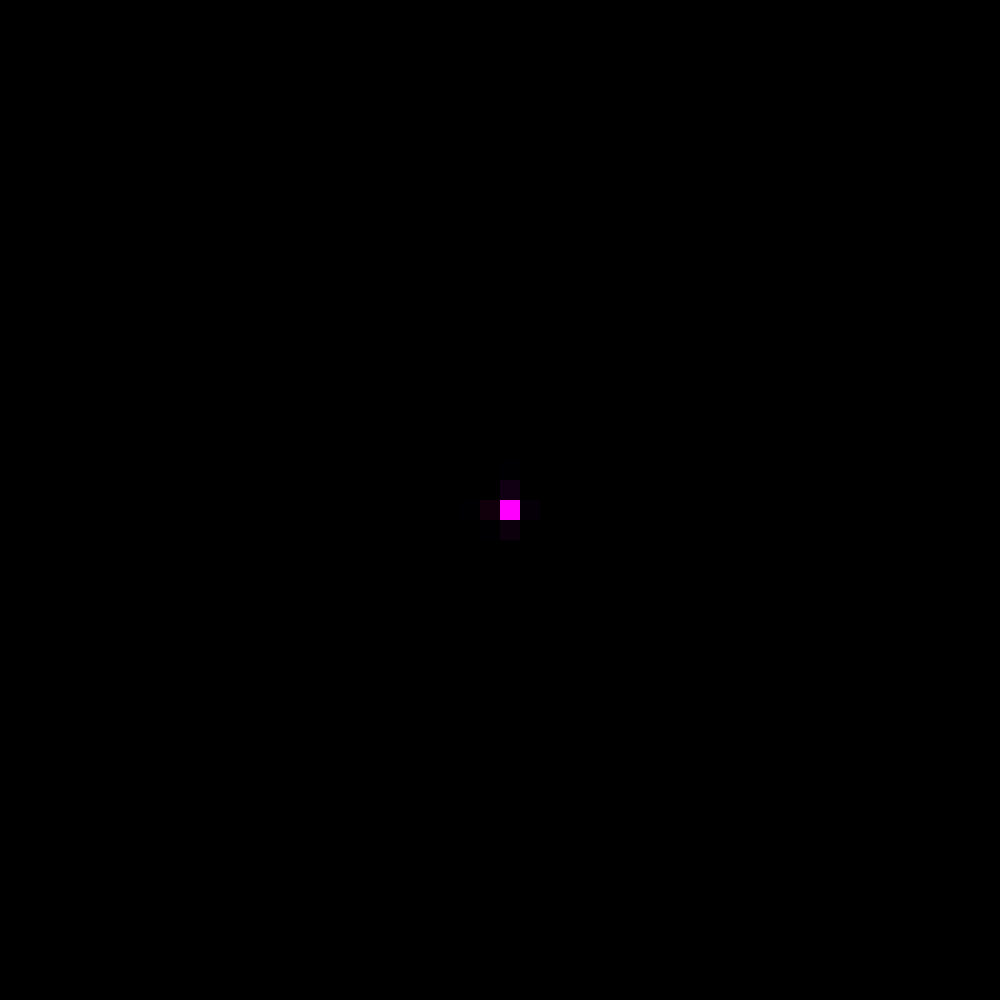
\includegraphics[height=0.8\textheight]{dsrd2d}}{dsrd2d.mp4}
\end{center}
}

\end{document}

